% Split-fill plot marks in a mathematical scatter plot.
\documentclass[border=2pt]{standalone}
\usepackage{pgfplots}
\usetikzlibrary{plotmarks}
\pgfplotsset{compat=newest}

\begin{document}
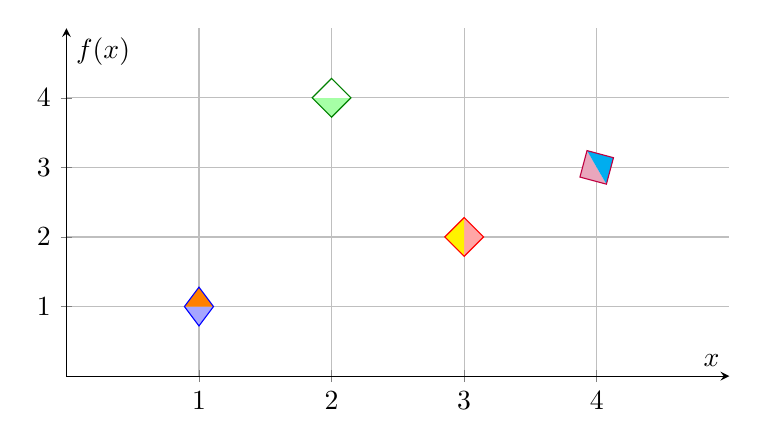
\begin{tikzpicture}
  \begin{axis}[
    width=10cm,height=6cm,
    xmin=0,xmax=5,ymin=0,ymax=5,
    axis lines=middle,grid=major,
    xlabel={$x$},ylabel={$f(x)$},
    xtick={1,2,3,4},ytick={1,2,3,4}
  ]
    \addplot[only marks,blue,fill=blue!35,mark color=orange,
      mark=halfdiamond*,mark size=7pt] coordinates {(1,1)};
    \addplot[only marks,green!50!black,fill=green!35,mark color=white,
      mark=halfsquare*,mark size=7pt] coordinates {(2,4)};
    \addplot[only marks,red,fill=red!35,mark color=yellow,
      mark=halfsquare right*,mark size=7pt] coordinates {(3,2)};
    \addplot[only marks,purple,fill=purple!35,mark color=cyan,
      mark=halfsquare left*,mark options={rotate=30},mark size=7pt]
      coordinates {(4,3)};
  \end{axis}
\end{tikzpicture}
\end{document}
